\documentclass[12pt]{article}
\usepackage{url, graphicx}
\usepackage{geometry}
\usepackage{amsmath}
\usepackage{fancyhdr}
\pagestyle{fancy}

\title{\huge Lecture 2: Recursive Algorithms: MergeSort; Binary Search; The Master Theorem; The Recursive Tree Method}
\author{}
\date{}
\pagestyle{fancy}
\fancyhf{}
\lhead{COMP 251 Winter 2018}
\rhead{Lecture 2}
\lfoot{$10^{th}$ Jan, 2018}
\rfoot{\copyright{}Yutong Yan}
\cfoot{\thepage}




\begin{document}
\maketitle
\section{Reductions and Sub-Routines}
\renewcommand{\labelitemii}{$\circ$}
\renewcommand{\labelitemiii}{$\cdot$}
\renewcommand{\labelitemiii}{$\rightarrow$}
\renewcommand{\labelitemiv}{$\star$}
\begin{itemize}
\item Solving a problem by \textbf{reducing} it (or a sub-problem of it) to another problem is the most fundamental technique in algorithm design.
\item Specifically, algorithm $A$ may use another algorithm $B$ as a sub-routine.
\item This has numerous advantages:
	\begin{itemize}
	\item \textbf{Code Verification}: the correctness of $A$ is independent of $B$.
	\item \textbf{Code Reuse}: a great time-saver.
	\end{itemize}
\item A simple but very powerful special case of this paradigm is when the algorithm calls itself!
	\begin{itemize}
	\item This method is called \textbf{recursion}.
	\end{itemize}
\end{itemize}

\section{MergeSort}
\renewcommand{\labelitemii}{$\circ$}
\renewcommand{\labelitemiii}{$\cdot$}
\renewcommand{\labelitemiii}{$\rightarrow$}
\begin{itemize}
\item We can sort n numbers into non-decreasing order using the following algorithm:\\
\\
{\large
\noindent MergeSort($x_1$, $x_2$, ... , $x_n$)\\
\noindent If n = 1 then output $x_1$\\
\noindent Else output Merge\{MergeSort($x_1$, ... , $x_{\frac{n}{2}}$), MergeSort($x_{\frac{n}{2} + 			1}$, ... , $x_n$)\} }\\
	\begin{center}
	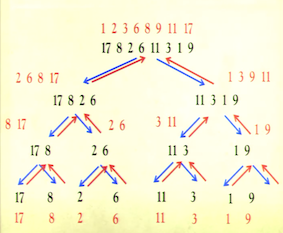
\includegraphics{lecture2a}
	\end{center} ~\newline
\item Two Problems:
	\begin{itemize}
	\item Does the algorithm work?\\
	\noindent Yes!
		\begin{itemize}
		\item The algorithm calls itself on smaller instances
			\begin{itemize}
			\item The division process terminates with a set of base cases of size 1.
			\end{itemize}
		\item MergeSort trivially works on the base cases. 
		\item So, given the validity of the Merge Step, the correctness of the algorithm follows by 				\textbf{strong induction}.
			\begin{itemize}
			\item As long as base case is correct and merge step works, everything will be fine.
			\end{itemize}
		\end{itemize}
	\item If so, is it efficient (polynomial time)?\\
	\noindent Yes! Look at the recursive formula.
		\begin{itemize}
		\item To analyze this we represent the running time $T$ (n) via a \textbf{recurrence}:\\
		\hspace*{\fill}\large{Recursive Formula: $T$(n) = 2 $\cdot$ $T$($\frac{n}{2}$) + c $\cdot$ n}\hspace*{\fill} 
			\begin{itemize}
			\item 2 $\cdot$ $T$($\frac{n}{2}$): Recuse on two problems with half the size.
			\item c $\cdot$ n: It takes linear time to merge two sorted lists.
			\end{itemize}
		\hspace*{\fill}\large{Base Case: $T$(1) = 1}\hspace*{\fill} 
			\begin{itemize}
			\item Or we can use $T$(c) = $O$(1) for any constant c.
			\end{itemize}
		\item The Running Time of MergeSort
			\begin{itemize}
			\item Theorem: MergeSort runs in time $O$(n $\cdot$ $\log{}n$)
			\item Proof: 
				\begin{enumerate}
				\item By adding dummy numbers, we may assume n is a power of two: n = 						$2^k$
				\item We can unwind the recursive formula as follows:\\
				\hspace*{\fill}\large{$T$(n) = 2 $\cdot$ $T$($\frac{n}{2}$) + c $\cdot$ n}\hspace*{\fill}
				\begin{center}
				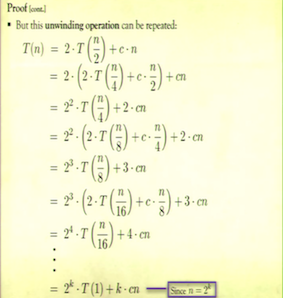
\includegraphics{lecture2b}
				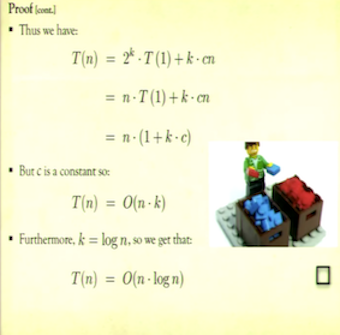
\includegraphics{lecture2c}
				\end{center}
				\end{enumerate}
			\end{itemize}
		\end{itemize}
	\end{itemize}
\end{itemize}


\section{Binary Search}
\renewcommand{\labelitemii}{$\circ$}
\renewcommand{\labelitemiii}{$\cdot$}
\renewcommand{\labelitemiii}{$\rightarrow$}
\renewcommand{\labelitemiv}{$\star$}
\begin{itemize}
\item We can search for a key k in a sorted array of cardinality n using the binary search algorithm:\\
\\
{\large
\noindent BinarySearch($a_1$, $a_2$, ... , $a_n$ : k)\\
\noindent While n $>$ 0 do: \\
		 If $a_{\frac{n}{2}}$ = k output YES\\
		 Else if $a_{\frac{n}{2}}$ $>$ k output BinarySearch($a_1$, $a_2$, ... , $a_{\frac{n}{2} - 			1}$ : k)\\
		Else if $a_{\frac{n}{2}}$ $<$ k output BinarySearch($a_{\frac{n}{2} + 1}$, ... , $a_n$: k)\\
		Output NO}
\begin{center}
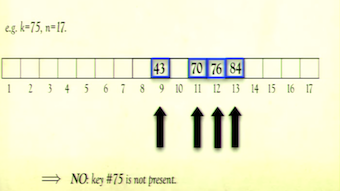
\includegraphics{lecture2d}
\end{center}
\item Does this work?
	\begin{itemize}
	\item The validity of the binary search follows simply by strong induction.(The base case is 		trivially true.)
	\end{itemize}
\item Running Time?
	\begin{itemize}
	\item Recurrence: 
	\begin{center}
	\large{Recursive Formula: $T$(n) = $T$($\frac{n}{2}$) + c} \\
	\large{Base Case: $T$(1) = 1}
	\end{center}
	\item Theorem: Binary Search runs in time $O$($\log{}n$)
	\begin{enumerate}
	\item By adding dummy numbers, we may assume n is a power of two: n = 					$2^k$
	\item We can unwind the recursive formula as follows:
	\begin{center}
	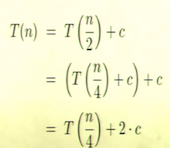
\includegraphics{lecture2e}
	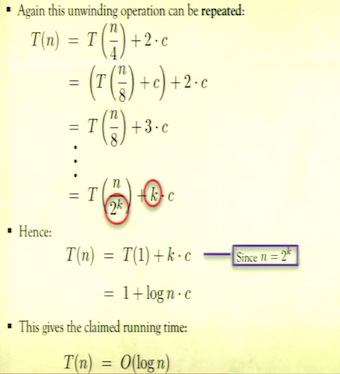
\includegraphics{lecture2f}
	\end{center}	
	\end{enumerate}
	\end{itemize}
\end{itemize}	
	
	
	
\section{Divide and Conquer Algorithms}
\renewcommand{\labelitemii}{$\circ$}
\renewcommand{\labelitemiii}{$\cdot$}
\renewcommand{\labelitemiii}{$\rightarrow$}
\renewcommand{\labelitemiv}{$\star$}
\begin{itemize}
\item A \textbf{divide and conquer} algorithm recursively breaks up a problem of size n in smaller sub-problems such that:
	\begin{itemize}
	\item There are exactly a sub-problems.
	\item Each sub-problem has size at most {\large $\frac{1}{b}$ $\cdot$ n}
	\item Once solved, the solutions to the sub-problems can be \underline{combined} to produce 	a solution to the original problem in time $O$($n^d$)
	\end{itemize}
\item So the run-time of a divide and conquer algorithm satisfies the recurrence:\\
\\
\hspace*{\fill}{\large $T$(n) = a $\cdot$ $T$($\frac{n}{b}$) + $O$($n^d$)} \hspace*{\fill} \\
\item MergeSort and Binary Search are indeed \textbf{divide and conquer} algorithms.
	\begin{center}
	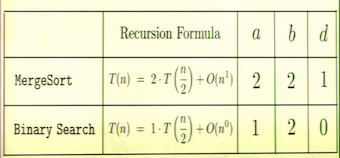
\includegraphics{lecture2g}
	\end{center}	
\end{itemize}



\section{Non-Military Applications of Divide and Conquer}
\renewcommand{\labelitemii}{$\circ$}
\renewcommand{\labelitemiii}{$\cdot$}
\renewcommand{\labelitemiii}{$\rightarrow$}
\renewcommand{\labelitemiv}{$\star$}
\begin{itemize}
\item Divide and Conquer has many other non-military, practical applications:
	\begin{itemize}
	\item Big Data
	\item Distributed Algorithms
	\item Clustering and Classification
	\item MapReduce
	\end{itemize}
\end{itemize}

\section{Dummy Entries}
\renewcommand{\labelitemii}{$\circ$}
\renewcommand{\labelitemiii}{$\cdot$}
\renewcommand{\labelitemiii}{$\rightarrow$}
\renewcommand{\labelitemiv}{$\star$}
\begin{itemize}
\item MergeSort actually has the recurrence:
	\begin{center}
	\large{$\hat{T}$(n) = $\hat{T}$([$\frac{n}{2}$]) + $\hat{T}$([$\frac{n}{2}$]) + c $\cdot$ n}
	\end{center}
\item Recall we got around this by adding dummy entries:
	\begin{itemize}
	\item We found $\hat{n}$ the smallest power of 2 greater than n.
	\item For this case, MergeSort then does have recurrence:
		\begin{center}
		\large{$T$(n) = 2 $\cdot$ $T$($\frac{n}{2}$) + c $\cdot$ n}
		\end{center}
	\item But we also have: 
		\begin{center}
		{\large $\hat{T}(n) \leq T(\bar{n}) = O(\bar{n} \cdot \log{}\bar{n}) = O(n \cdot \log{}n) $}
		\end{center}
	\end{itemize}
\item Here is another way to solve the recurrence:
	\begin{center}
	{\large $\hat{T}(n) = \hat{T}([\frac{n}{2}]) + \hat{T}([\frac{n}{2}]) + c \cdot n$}
	\end{center}
	\begin{itemize}
	\item As we only want to upper bound the running time, we can use:
	\begin{center}
	{\large $\hat{T}(n) \leq \hat{T}(\frac{n}{2} + 1) + c \cdot n$}
	\end{center}
	Note: This +1 does not seem to fit with our methodology, but we can fix this by applying a 			\textbf{domain transformation}.
	\end{itemize}
\item Domain Tranformation
	\begin{itemize}
	\item For the domain transformation, simply set: {\large $T$(n) = $\hat{T}$(n + 2)}
	\item Thus we have: {\large $T$(n) = $T$(${\frac{n}{2}}$) + $\hat{c}$ $\cdot$ n}
		\begin{center}
		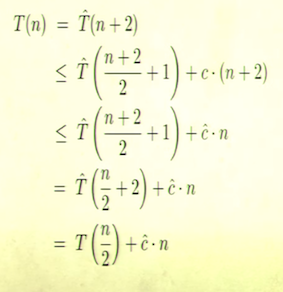
\includegraphics{lecture2l}
		\end{center}
	\item Of course, we can solve this recurrence as: {\large $T$(n) = $O$(n $\cdot$ $\log{}n$)}
	\item Therefore, {\large $\hat{T}$(n) = $T$(n - 2) = $O$(n $\cdot$ $\log{}n$)}
	\item As well as ceilings and floors, domain transformations can be used to 
	$\underline{simplify}$ many other recurrences; e.g. removing lower order terms.
	\end{itemize}
\end{itemize}

\end{document}